% !TeX encoding = UTF-8
\documentclass[12pt, a4paper]{article}
% \title{Дифракция света на ультразвуковой волне (4.3.2)}
% \author{Струков Олег, Б04-404}
% \date{}
\usepackage{geometry}
\usepackage{amsmath, amsfonts, amssymb, amsthm} % стандартный набор AMS-пакетов для математ. текстов
\usepackage{mathtext}
\usepackage[utf8]{inputenc} % кодировка utf8
\usepackage[russian]{babel} % русский язык
\usepackage[pdftex,dvipsnames]{xcolor} % работа с цветами
\usepackage[pdftex]{graphicx} % графика (картинки)
\usepackage{tikz,pgfplots} % рисунки
\usepackage{indentfirst}
%\usepackage[labelfont=bf,labelsep=endash,skip=3pt]{caption} % подпись картинок
% \usepackage{fancyhdr,pageslts} % настройка колонтитулов
\usepackage{enumitem} % работа со списками
\usepackage{floatrow,multicol,multirow,longtable,hhline} % работа с таблицами
\usepackage{float,wrapfig} % плавающие объекты
\usepackage{tcolorbox} % рамка вокруг текста
%\usepackage[calc]{datetime2} % дата
\usepackage{bm} % жирное начертание в формулах
\usepackage{physics} % физический пакет
\DeclareMathAlphabet\mathbfcal{OMS}{cmsy}{b}{n}
\usepackage{pgfornament} % красивые рюшечки и вензеля
\usepackage{mdframed}
\usepackage{derivative}
\usepackage{mathrsfs} %EDS
\usepackage{soul} % strikethorugh
%\usepackage{boondox-cal}

% ----------------------------------------
% Настройка шрифта

% Просто закооментируйте следующую строчку, если не работает. Будет другой шрифт, правда :(
% \usepackage{pscyr}

% ----------------------------------------
% Стилевые настройки

\usepackage{boldline} % жирная линия после таблиц (чтобы не было ошибок, этот пакет должен подключаться именно тут!)
\floatsetup[table]{style=Plaintop,floatrowsep=qquad} % настройка оформления таблиц
\setlist[enumerate,itemize]{leftmargin=5mm,itemindent=10mm,itemsep=0mm,
listparindent=0em,labelsep=2mm,topsep=2mm,labelwidth=4mm} % настройки списков

\setlength{\columnsep}{0.5cm} % расстояние между колонками
\setlength{\parskip}{1pt} % расстояние до текста от колонтитула

%\usepackage{titlesec} % управление оформлением section
%\renewcommand{\thesection}{\Roman{section}}
%\titleformat{\section}[block]{\bfseries\large}{\thesection.}{5pt}{}

% Настройка совместимости
\pgfplotsset{compat=1.18}

% ----------------------------------------
% Настройки полей
\geometry{
	left=10mm,
	top=10mm,
	right=10mm,
	bottom=15mm,
	marginparsep=0mm,
	marginparwidth=0mm,
	headheight=0pt,
	headsep=0pt,
	footskip=20pt}

% ----------------------------------------
% Настройки колонтитулов и нумерации страниц
\pagenumbering{arabic}



\newcounter{ntask}
\setcounter{ntask}{0}


\newcommand{\arsh}{\mathrm{arsh} \,\,}
\newcommand{\arch}{\mathrm{arch} \,\,}
\newcommand{\arth}{\mathrm{arth} \,\,}
\newcommand{\arcth}{\mathrm{arcth} \,\,}
\renewcommand{\Re}{\operatorname{Re} \,}
\newcommand{\EDS}{\mathscr{E}}
\newcommand{\diffract}[1]{\frac{\mathrm{d}#1}{\mathrm{d}t}}

\newcommand{\kHz}{~\mathrm{kHz}}
\newcommand{\GHz}{~\mathrm{GHZ}}
\newcommand{\us}{~\mathrm{\mu s}}
\addto\captionsrussian{\def\refname{Источники}}

\begin{document}
\title{\begin{center}Лабораторная работа № 4.3.2\end{center}
Дифракция света на ультразвуковой волне}
\author{Струков О. И. \\ Б04-404}
\date{}

\thispagestyle{empty}
\pagenumbering{gobble}
\maketitle
\newpage
\pagenumbering{arabic}

\section*{Введение}
\textbf{Цель:} изучение дифракции света на синусоидальной акустической решётке и наблюдение фазовой решётки методом тёмного
поля.

\textbf{В работе используются :} оптическая скамья, осветитель, два длиннофокусных объектива, кювета с жидкостью, кварцевый излучатель
с микрометрическим винтом, генератор ультразвуковой частоты, линза, вертикальная нить на рейтере, микроскоп.

\section*{Теоретическая часть}
При прохождении ультразвуковой волны через жидкость в ней возникают периодические неоднородности коэффициента преломления, создается фазовая решетка, которую мы считаем неподвижной ввиду малости скорости звука относительно скорости света. Показатель
	преломления n изменяется по закону:
	
	\begin{equation}\label{}
	n = n_0 (1 + m \cos \Omega x)
	\end{equation}
	
	Здесь $ \Omega = 2 \pi / \Lambda $ --- волновое число для ультразвуковой волны, $ m $ --- глубина модуляции $ n $ $ (m \ll 1 $).
	
	Положим фазу $ \phi $ колебаний световой волны на передней стенке кюветы равной нулю, тогда на задней поверхности она равна:
	
	\begin{equation}\label{}
	\phi  = k n L = \phi_0 (1 + m \cos \Omega x)
	\end{equation}
	
	Здесь $ L $ -- толщина жидкости в кювете, $ k = 2 \pi / \lambda $ --- волновое число для света.
	
	После прохождения через кювету световое поле есть совокупность плоских волн, распространяющихся под углами $ \theta $, соответствующими максимумам в дифракции Фраунгофера:
	
\begin{equation}\label{}	
	\Lambda \sin \theta_m = m \lambda
\end{equation}

Этот эффект проиллюстрирован на рисунке 1.

	Зная положение дифракционных максимумов, по формуле (1) легко определить длину ультразвуковой волны, учитывая малость $ \theta $: $ \sin \theta \approx \theta \approx l_m /F  $, где $ l_m $ --- расстояние от нулевого до последнего видимого максимума, $ F $ --- фокусное расстояние линзы. Тогда получим:
	
	\begin{equation}\label{}
	 \Lambda = m \lambda F/ l_m 
	\end{equation}
	Скорость ультразвуковых волн в жидкости, где $ \nu $ -- частота колебаний излучателя:
	
\begin{equation}\label{}
	v = \Lambda \nu 
\end{equation}

\begin{figure}[H]
	\center{
\includegraphics[scale=1]{1.jpg}}
  \caption{Эффект дифракции на ультразвуковой волне}
\end{figure}

\section*{Экспериментальная установка}
Источник света Л с помощью конденсора К проецируется на входную (коллиматорную) щель $S$. Входная щель ориентирована горизонтально и прикрыта красным светофильтром Ф. Коллиматорный объектив $\text{О}_1$ посылает параллельный пучок на кювету с водой $С$. Излучатель Q создаёт УЗ-волну. Параллельный пучок света, дифрагируя на стоячей звуковой волне, образует дифракционную картину в фокальной плоскости $F$ камерного объектива $\text{О}_{2}$. Картину можно наблюдать в микроскоп М.
\begin{figure}[H]
	\center{
\includegraphics[scale=1]{2.jpg}}
  \caption{Схема экспериментальной установки}
\end{figure}
% \begin{figure}[H]
%   
\includegraphics[width=0.8\linewidth]{setup.png}
%   \caption{Схема установки}
% \end{figure}

\begin{figure}[H]
  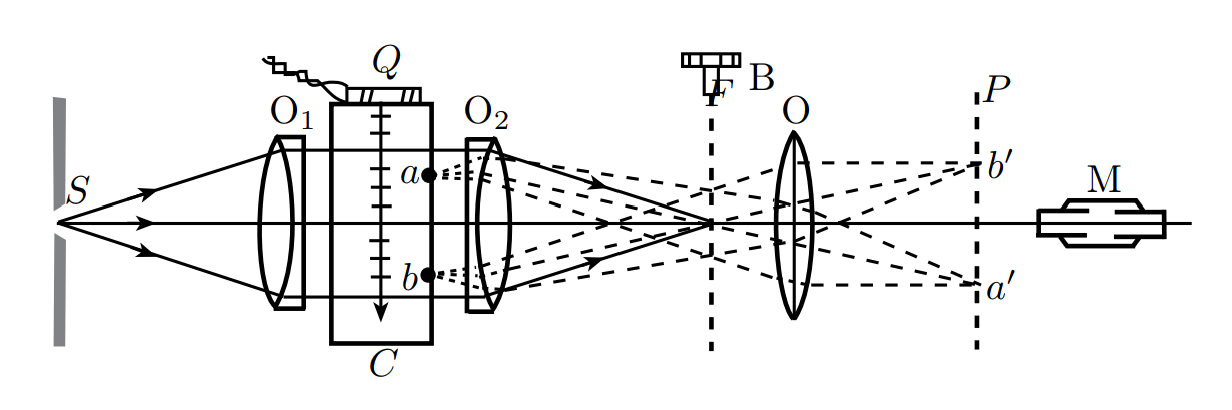
\includegraphics[width=0.8\linewidth]{setup-2.png}
  \caption{Схема установки для измерения методом тёмного поля}
\end{figure}
Теперь получим изображение фазовой решётки. Для этого используем метод <<тёмного поля>> -- 
закрывания центрального максимума в дифракционной картине с помощью тонкой нити и на рейтере. 
В поле зрения микроскопа при этом образуется изображение фазовой решётки с шириной линии
$\Lambda/2$, где $\Lambda$ -- длина УЗ-волны в воде.

Данные об установке:
\begin{itemize}
  \item \textbf{Фокусное расстояние линзы O2 }$f = 28$ см;
  \item \textbf{Длина волны }$\lambda = (640\pm20)$ нм.
\end{itemize}

\section*{Ход работы}
\subsection*{Определение скорости ультразвука по дифракционной картине}
На настроенной по схеме на рисунке 2 установке была получена дифракционная картина, на которой отчётливо было видно 7 дифракционных полос.

При частоте генератора 1,03 МГц по опусканию излучателя было определено, что длина половины волны составляет примерно 220 мкм. Отсюда была получена оценка скорости ультразвука в воде: $v = \lambda \nu \sim 453$ м/с, что достаточно далеко от табличного значения 1497 м/с.

Далее при различных частотах с помощью перекрестия и микрометрического винта на выходе из прибора были определены координаты Y каждой светлой полосы.
По полученным результатам построен график зависимости Y(m), найдены коэффициенты наклона прямых, и с их помощью рассчитана скорость ультразвука в воде:

\[ \Lambda = \dfrac{m f \lambda}{l_m}, \qquad v = \lambda \nu = \dfrac{\lambda f \nu m}{l_m} \]

\begin{figure}[H]
  
\includegraphics[width=1\linewidth]{1.pdf}
\end{figure}

\begin{table}[H]
  \centering
\begin{tabular}{|l| c|c|c|c|}
\hline
$\nu$, МГц & 1,044 & 1,248 & 1,504 & 2,014 \\ \hline
$k$, мкм   & 132,4 & 163,2 & 175,2 & 270 \\ \hline
$\Lambda$, мм &1,353&	1,098&	1,023&	0,664
 \\ \hline
$v$, м/с   & 1413,03 & 1370,76 & 1538,34 & 1336,70 \\
\hline
\end{tabular}
\end{table}

Среднее значение скорости с учётом погрешности составило $v_{\text{ср}} = (1415 \pm 76)$ м/с, что существенно ближе к табличному по сравнению с первым оценочным результатом.





















% Для начала получим дифракционную картину. Отчётливо видны отдельные полосы, при этом при увеличении
% мощности генератора полос становится заметно больше (вплоть до 11).

% Снимем зависимость отсчётов микрометрического винта в зависимости от номера полосы, а также частоты
% генератора:
% \begin{table}[H]
%   \centering
%   \begin{tabular}{|c|c|}
%       \hline
%       Частота ($\text{МГц}$) & Отсчёты \\ \hline
%       1.07188 & 11, 53, 86, 125, 164, 203, 240 \\ \hline
%       1.19215 & 69, 113, 155, 191, 233, 279, 326, 365, 409 \\ \hline
%       1.24837 & 0, 39, 76, 119, 164 \\ \hline
%       2.89424 & 36, 141, 244, 345, 449, 554, 656 \\ \hline
%       4.83451 & 75, 248, 418 \\ \hline
%   \end{tabular}
%   \caption{Зависимость счетчиков от частоты.}
%   \label{freq_counts_table}
% \end{table}
% Принимаем во внимание, что один отсчёт винта соответсвует $4~\mathrm{\mu m}$.
% Найдём тогда линеаризацией соответсвующие ширины дифракционных полос:
% % \begin{figure}[H]
% %   \includegraphics[width=0.75\linewidth]{line count.png}
% % \end{figure}
% Тогда справедливо следующее:
% $$\Lambda = v/f, \quad h(f) \approx F_2 \cdot \theta(f) = F_2 \cdot \lambda/\Lambda = \lambda F_2 f / v \quad(\theta \ll 1)$$
% $$h = \frac{\lambda F_2}{v} f$$
% Согласно данной зависимости линеаризуем:
% % \begin{figure}[H]
% %   \includegraphics[width=0.75\linewidth]{pics/speed_of_sound_1.png}
% % \end{figure}
% И получаем значение $v = \lambda F_2 / k = (1250\pm60)~\mathrm{m/s}$,
% что вообще-то достаточно далеко от табличного значения в $1490~\mathrm{m/s}$...

\subsection*{Измерение методом тёмного поля}
Для измерения скорости ультразвука методом тёмного поля центральный максимум был закрыт проволокой, а шкала микроскопа откалибрована -- 1 мм на ней соответствует 39 делениям шкалы. 


\begin{table}[H]
\centering
\begin{tabular}{|c|c|c|}
\hline
Частота, МГц & Расстояние, дел. & $\Lambda$, мм \\
\hline
1,139   & 0,2695      & 1,378 \\ 
1,438   & 0,238       & 1,218 \\
1,476   & 0,231      & 1,186 \\
1,629   & 0,208      & 1,068 \\
1,694   & 0,200          & 1,026 \\
1,778   & 0,188       & 0,962 \\
2,085   & 0,160         & 0,821 \\
\hline
\end{tabular}
% \caption{Зависимость параметров от частоты}
\label{tab:data}
\end{table}

Построен график зависимости $\Lambda (1/\nu)$:

\begin{figure}[H]
  
\includegraphics[width=1\linewidth]{2.pdf}
\end{figure}

По наклону прямой определена скорость ультразвука в воде $v = (1419\pm110$ м/с.

В случае закрытия проволокой боковых максимумов на изображении возникают аналогичные полоски, выраженные более слабо.





% При нормировке собственной шкалы микроскопа по линейке, на которую он сфокусирован, оказалось, что
% 1 мм линейки соответсвует ($15.5\pm0.5$)делениям шкалы.

% Ввиду количества данных, они сразу приведены в графическом виде для удобства.
% % \begin{figure}[H]
% %   \includegraphics[width=0.75\linewidth]{pics/dark field.png}
% % \end{figure}

% По полученным данным рассчитаем соотвествующие скорости звука в воде:
% \begin{table}[H]
%   \begin{tabular}{|l|l|l|l|}
%   \hline
%   f, MHz & H, a.u. & $H_\text{toscale}$, mm & $v$, m/s \\ \hline
%   1.0999 & 10.57   & 0.705          & 1500   \\ \hline
%   1.2494 & 9.15    & 0.610          & 1474   \\ \hline
%   2.8798 & 3.96    & 0.264          & 1470   \\ \hline
%   \end{tabular}
% \end{table}

% Таким образом, этим методом получено $v = (1480\pm50)~\mathrm{m/s}$, что уже гораздо лучше совпадает с табличным значением.
\section*{Вывод}
В данной работе были получены дифракционные картины на стоячей волне сжатия в воде, а так же
изображение фазовой решётки методом тёмного поля. Были получены оценки скорости ультразвуковых волн
в воде, близкие к табличному значению: 1415 м/с в первом случае и 1419 м/с во втором, причём во втором случае табличное значение 1497 м/с находится в пределах погрешности рассчитаного.
\end{document}